\section{Bestapproximation (BA)}
Aufgabenstellung:\\
Gegeben:
\begin{itemize}
  \item Element $f \in H$ (z.B. Funktion in $C[a,b]$)
  \item Raum $U$ für die Approximation (z.B. $\Pi_n$)
  \item Norm $\norm{.}$
\end{itemize}
Gesucht:
Bestapproximation $g \in U$ von $f$ bezüglich $\norm{.}$, so dass 
\begin{align*}
  \norm{f - g} \leq \norm{f - u}\,\forall\,u \in U
\end{align*}

\subsection{BA bezgl. einer durch ein Skalarprodukt induzierten Norm}
\para{Satz} Sei $H$ ein Vektorraum und $\inner{.}{.}$ ein Skalarprodukt auf $H$, das die
Norm $\norm{.}$ induziere. Weiters sei $U$ ein endlichdimensionaler Unterraum von $H$.
Dann gilt:
\begin{enumerate}[a)]
  \item $g \in U$ ist BA von $f$ bzgl. 
    $\norm{.}\,\Longleftrightarrow\,\inner{f - g}{u} = 0\,\forall\,u \in U$
    (Orthogonalitätseigenschaft)
  \item $\forall f \in H$ gibt es genau eine BA $g \in U$ bzgl. $\norm{.}$
\end{enumerate}
Beweis: a) Einsetzen und Umformen
\begin{figure}[htbp]
  \centering
  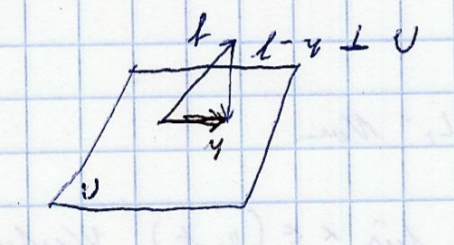
\includegraphics[width=0.3\textwidth]{figures/ba_ebene.png}
  \label{Darstellung auf Ebene}
\end{figure}\\
Beweis: b) (Wir führen den Bewis für $\mathbb{K} = \mathbb{R}$;
Analoger Beweis für $\mathbb{K} = \mathbb{C}$)\\
Konstruktionsbeweis: Sei ${\phi_0,\,\ldots,\,\phi_n}$ eine Basis von $U$ und $f \in H$\\
Ansatz: $g = \sumzn{j}{a_j \phi_j}$, wobei wir zeigen, dass $\ztoxn{a}$
eindeutig bestimmt sind, so dass $g$ BA von $f$ bzgl. $\norm{.}$ ist.
Teil a)
\begin{align*}
  g \in U \text{ ist BA von } f &\Longleftrightarrow \inner{f - g}{u} = 0\, \forall\, u \in U\\
  &\Longleftrightarrow\\
  \inner{f-g}{\phi_i} &= 0\, \forall\, i=0,\,\ldots,\,n\\
  &\Longleftrightarrow\\
  \inner{g}{\phi_i} &= \inner{f}{\phi_i}\, \forall\, i=0,\,\ldots,\,n\\
  \sumzn{j}{a_j\inner{phi_j}{\phi_i}} &= \inner{f}{\phi_i}\, \forall\, i=0,\,\ldots,\,n\\
  a_0\inner{\phi_0}{\phi_0} + a_1\inner{\phi_1}{\phi_0} + \ldots + a_n\inner{\phi_n}{\phi_0} &= \inner{f}{\phi_0}\\
    a_0\inner{\phi_0}{\phi_1} + a_1\inner{\phi_1}{\phi_1} + \ldots + a_n\inner{\phi_n}{\phi_1} &= \inner{f}{\phi_1}\\
  \ldots\\
  a_0\inner{\phi_0}{\phi_n} + a_1\inner{\phi_1}{\phi_n} + \ldots + a_n\inner{\phi_n}{\phi_n} &= \inner{f}{\phi_n}\\
  &\Longleftrightarrow\\
  M\underline{a} &= \underline{f}
\end{align*}
\begin{align*}
  M[i,j] &= \inner{\phi_j}{ \phi_i}\; i,j = 0,\,1,\,\ldots,\,n\\
    \underline{f}[i] &= \inner{f}{ \phi_i}\; i = 0,\,1,\,\ldots,\,n\\
  \underline{a}[i] &= a_i\; i = 0,\,1,\,\ldots,\,n\\
\end{align*}
M nennt man Gramsche Matrix zu $\ztoxn{\phi}$\\
Es bleibt z.z.: $M$ ist invertierbar.\\
Sei $\underline{b} \in \mathbb{R}^{n+1} \setminus \{\underline{0}\}$
\begin{align*}
  (M \underline{b})[i] &= \sumzn{j}{\inner{\phi_j}{\phi_i}b_j} = \sumzn{j}{\inner{b_j\phi_j}{\phi_i}}\\
  \inner{M \underline{b}}{\underline{b}}_2 &= \sumizn{\inner{\sumzn{j}{b_j\phi_j}}{\phi_i}b_i}\\
  &= \inner{\underbrace{\sumzn{j}{b_j\phi_j}}_{a \in U}}{\underbrace{\sumizn{b_i\phi_i}}_{a \neq 0}}\\
  &= \inner{a}{a} > 0
\end{align*}
$\Rightarrow\,M$ ist positiv definit (siehe später), d.h. alle Eigenwerte von $M$ sind positiv.\\
$\Rightarrow\,M$ ist invertierbar.\\
Praktische Vorgangsweise zur Bestimmung der BA $g \in U$ von $f$ bzgl. $\norm{.}$ bzw. $\inner{.}{.}$
\begin{enumerate}
  \item Bestimme geeignete Basis $\phi_0,\ldots,\phi_n \in U$
  \item Ansatz: $g = \sumzn{j}{a_j\phi_j}$ wobei $a_0,\ldots,a_n$ bestimmt werden durch 
    $\sumzn{j}{a_j\inner{\phi_j}{\phi_i}} = \inner{f}{\phi_i}\,i=0,\ldots,n$
\end{enumerate}
Eine explizite Darstellung der BA lässt sich angeben, wenn die gewählte Basis
ein Orthogonalsystem für $U$ bildet, d.h.
\begin{align*}
  \inner{\phi_j}{\phi_i} \begin{cases}
    = 0 &\mbox{für } j \neq i\\
    \neq 0 &\mbox{für } j = i
  \end{cases}
\end{align*}
$\Rightarrow \sumzn{j}{a_j\inner{\phi_j}{\phi_i}} = a_i \inner{\phi_i}{\phi_i} = \inner{f}{\phi_i}\,i=0,\ldots,n$\\
$\Rightarrow g = \sumzn{j}{\frac{\inner{f}{\phi_j}}{\inner{\phi_j}{\phi_j}} \phi_j}$ TODO stimmt des so?

\subsubsection{BA durch Polynome in der gewichteten L2-Norm}
\para{Definition:} Sei $\omega: (a,b)\longrightarrow \mathbb{R}$ stetig, $\omega(x) > 0$ für $x \in (a,b)$.
Weiters sei $\omega$ zumindest uneigentlich integrierbar auf $(a,b)$. $\omega(x)$ ist eine Gewichtsfunktion.
\begin{align*}
  \inner{f}{g}_\omega &:= \int_a^b \omega(x) f(x)g(x) \dx\\
  \norm{f}_\omega &:= \sqrt{\int_a^b \omega(x) [f(x)]^2 \dx}
\end{align*}
(Wir betrachten nur reellwertige Funktionen)\\
Aufgabenstellung:\\
Gegegeben: $f \in C[a,b],\,n \in \mathbb{N}_0,\,\norm{.}_\omega$\\
Gesucht: $p_n \in \Pi_n:\,\norm{p_n - f} \leq \norm{q_n - f}\,\forall\, q_n \in \Pi_n$

Ansatz über Orthogonalpolynome $\rightarrow$ Gram-Schmidt Orthogonalisierungsverfahren
für $\psi_0,\ldots,\psi_n$ Basis von $U$
\begin{align*}
  k &= 0 & \phi_0 &= \psi_0\\
  k &\mapsto k+1 & \phi_{k+1} &= \psi_{k+1} - \sum\limits_{i=0}^{k}{\frac{\inner{\psi_{k+1}}{\phi_i}}{\inner{\phi_i}{\phi_i}}\phi_i}
\end{align*}
$\Rightarrow \phi_0,\ldots,\phi_n$ ist orthogonale Basis von $U$ (Einsetzen)\\
``Günstigeres'' Orthogonalisierungsverfahren für Polynome über ``Dreiterm-Rekrsuion'', siehe z.B. Wikipedia.\\
Beispiel: Orthogonalpolynome für $\omega \equiv 1$ und $[a,b]=[-1,1]$ sind die Legendre-Polynome:
\begin{align*}
  P_0(x)\equiv 0, \, P_1(x)=x, \, P_2(x)=x^2 - \frac{1}{3},\ldots
\end{align*}
Beispiel: Orthogonalpolynome bzg. $\omega(x)=\frac{1}{\sqrt{1-x^2}}$ und $[a,b]=[-1,1]$ sind die Tschebyscheff-Polynome.\\
\para{Satz:} Sei $f \in C^k[a,b]\, k \in \mathbb{N}$ und $p_n \in \Pi_n$ sei die BA von f bzgl. der L2-Norm. Dann gilt:
\begin{align*}
  \norm{f-p_n}_{L2} \leq C(k,f)n^{-k} \underset{n \to \infty}{\longrightarrow} 0
\end{align*}

\subsubsection{BA durch stückweise lineare Funktionen bezüglich $\norm{.}_{L2}$}
Gegeben: $f$ in $[a,b]$ und $a=x_0<x_1<\ldots<x_n=b$\\
Gesucht: $s_L \in S_L$ BA von $f$ bzgl. $\norm{.}_{L2}$\\
Anstatt einer Orthogonalbasis werden die Hutfunktionen $\phi_0,\ldots,\phi_n$ als Basis von $S_L$ verwendet.
Die Hutfunktionen sind ``fast orthogonal'', denn
\begin{align*}
  \inner{\phi_j}{\phi_i}_{L2} = \int_a^b \phi_i(x)\phi_j(x)\dx\begin{cases}
    =0 &\mbox{für } \abs{i-j} \geq 2\\
    \neq0 &\mbox{für } \abs{i-j} \leq 1\\
  \end{cases}
\end{align*}
\begin{figure}[htbp]
  \centering
  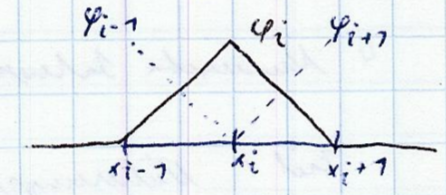
\includegraphics[width=0.3\textwidth]{figures/hutfunktionen2.png}
  \label{Hutfunktionen}
\end{figure}
Berechnung von $s_L$:\\
Ansatz: $s_L(x)=\sumzn{j}{a_j \phi_j(x)}$, wobei $a_0,\ldots,a_n$ bestimmt werden durch:
\begin{align*}
  s_L \mbox{ ist BA von } f &\Leftrightarrow \inner{s_L - f}{\phi_i} = 0 \mbox{ für } i=0,\ldots,n\\
  &\Leftrightarrow \sumzn{j}{a_j\inner{\phi_j}{\phi_i}} = \inner{f}{\phi_i}\mbox{ für } i=0,\ldots,n\\
  &\Leftrightarrow M \underline{a} = \underline{f}
\end{align*}
$M$ (Gramsche Matrix, Massenmatrix) $\in \mathbb{R}^{(n+1)\times(n+1)}$
\begin{align*}
  M[i,j] &= \inner{\phi_j}{\phi_i}_{L2} = \int_a^b \phi_j(x)\phi_i(x) \dx\\
  M[i,j] &= 0 \mbox{ für } \abs{i-j} \geq 2
\end{align*}
\begin{align*}
  n &= 1 & M &= \frac{1}{6}\begin{pmatrix}
    2h_1 & h_1\\
    h_1 & 2h_1
  \end{pmatrix}\\
  n &> 1 & M &= \frac{1}{6}\begin{pmatrix}
		      2 h_1   & h_1 &        &          & &  \\
					h_1     & 2(h_1+h_2)   & h_2      & &  \\
                  & h_2          & \ddots   & h_{n-1} & \\
                  &              &  h_{n-1} & 2(h_{n+1}+h_n)  & h_n \\
									&              &  & h_n   & 2 h_n
		      \end{pmatrix}
\end{align*}
$h_i = x_i - x_{i-1}\,\,i=1,\ldots,n$
\para{Satz:} Sei $s_L \in S_L$ die BA von $f \in L2(a,b)$ bzgl. $\norm{.}_{L2}$
\begin{enumerate}[(a)]
  \item Ist $f' \in [a,b]$: $\norm{f-s_L}_{L2} \leq \frac{1}{\sqrt{2}} h_{max} \norm{f'}_{L2}$
  \item Ist $f'' \in L2(a,b)$: $\norm{f-s_L}_{L2} \leq \frac{1}{2} h^2_{max} \norm{f''}_{L2}$
    %TODO is it possible to align them?
\end{enumerate}
Beweis: Nicht schwierig, siehe Hanke\\
Eine bessere Abschätzung bzgl. $h_{max}$ als in (b) ist nicht möglich.
Auch durch Interpolation wird ein Fehler von $\LandauO(h^2_{max})$ erreicht,
wenn $f'' \in L2(a,b)$ ist; siehe Hanke.

\subsection{BA bzgl. einer nicht durch ein Skalarprodukt induzierten Norm}
Beispiel: $\norm{.}_\infty$
Für Approximationen in endlichdimensionalen Räumen gilt:
\begin{itemize}
  \item Es existiert eine BA, sie muss aber nicht eindeutig sein.
  \item Es gibt i.A. keine geschlossene Darstellung einer BA.
  \item Für $f \in C[a,b]$ und für $\norm{.}_\infty$ gilt:
    \begin{itemize}
      \item Es existiert eine eindeutig bestimmte BA in $\Pi_n$
      \item Es gibt i.A keine geschlossene Darstellung. Iterativer Renz-Algorithmus liefert BA
        $\rightarrow$ aufwändig und BA ist nur unwesentlich besser als die ``Tschebyscheff-Interpolation'',
        siehe Kapitel~\ref{ch:interpolation}.
    \end{itemize}
\end{itemize}
